% !TEX root = ../my-dissertation.tex
%
\chapter{Experimental apparatus}
\label{sec:experiment}

\section{Introduction}
\label{sec:experiment:introduction}
Scattering experiments have been the key to furthering our understanding of the elementary constituents of matter and their interactions. The seminal work of Geiger, Marsden, and Rutherford~\cite{Geiger_1908} on the scattering of \(\alpha\)-particles%
\footnote{The kinetic energy of the \(\alpha\)-particles used in Rutherford's experiment is \SI{8}{\mega\electronvolt}. Modern particle accelerators achieve millionfold beam energy of \SI{6.5}{\tera\electronvolt}.} %
from thin metal foils in 1908 unravelled the structure of the atom and led to the discovery of the atomic nucleus.
Today, scattering experiments have evolved to using the very same atomic nuclei discovered over a century ago as probes for the uncharted frontiers of particle physics.

The natural observable of scattering experiments is the cross-section \(\sigma\)~\cite{Thomson2013}. In a classical interpretation, the number of scattered objects is related to the cross-sectional area of a scattering object, which allowed Rutherford to deduce the size of the atomic nucleus. However, the quantum nature of elementary particles ultimately only allows for a probabilistic description of nature by predicting the probability for a process to happen. In this interpretation, the cross-section has a more abstract meaning as a measure of the interaction strength. It is related to the underlying theory by the equation~\cite{Schwartz2013}
\begin{align}
    \sigma = \frac{1}{\Phi_{i}} \int \abs{\bra{f} \mathcal{M} \ket{i}}^2 \dd{\Pi}_{f}.
\end{align}
Here, \(\Phi_{i}\) is the flux of initial state particles \(\ket{i}\) and \(\dd{\Pi}_{f}\) is the differential kinematically allowed phase space of the final states \(\ket{f}\). The modulus square of the matrix element \(\bra{f} \mathcal{M} \ket{i}\) gives the probability \(P(\ket{i} \rightarrow \ket{f})\) for a transition from \(\ket{i}\) to \(\ket{f}\). The preparation of initial states \(\ket{i}\) and measurement of final states \(\ket{f}\) dictates the experimental setup of a scattering experiment with the aim of empirically testing the underlying theory and exploring the structure of matter.

The momentum of initial states \(\ket{i}\) determines the scale on which nature can be investigated\footnote{The de Broglie relation \(\lambda = 1 / p\) relates the momentum \(p\) of a probe with the size of the structure that can be resolved.}.
Rays of particles with considerable momentum and consequently smaller wavelength allow probing structures on more minor length scales.
Although cosmic rays from astrophysical sources can achieve ultra-relativistic energies up to \SI{e20}{\electronvolt}, their rate is vanishingly small~\cite{Gaisser2016}, so that one can only hope for their detection by terrestrial experiments.

The invention of modern particle accelerators marked a turning point. Particle accelerators not only allow for a reproducible preparation of initial states \(\ket{i}\) in a controlled laboratory environment but also their production in abundant number.
Remarkably, the kinetic energy of colliding particles also determines the mass scale of the particles created in the collision, possibly giving access to previously inaccessible heavy states. As their production cross-section often is small, only particle accelerators can produce these heavy states in sufficient quantities to allow for their observation.
In summary, in a modern scattering experiment, particle accelerators prepare the initial states \(\ket{i}\).
The two defining quantities of equal importance for a collider experiment are the energy and the rate of collision events.
The total beam energy in the centre-of-mass frame \(\sqrt{s}\) is the first defining characteristic of particle accelerators. High centre-of-mass energy is required for probing the structure of matter at smallest scales and for producing yet unobserved heavy states.
The luminosity is the second defining characteristic of a collider experiment. The number of scattering events measured in a collider experiment for a process with cross-section \(\sigma\) during a time \(\Delta T\) is
\begin{align}
    N =  \sigma \cdot \int\limits_{\Delta T} \dd{T} L_{\text{inst}} = \sigma \cdot L.
\end{align}
It is determined by the instantaneous luminosity \(L_{\text{inst}}\).  The amount of collected data is quantified by the integrated luminosity \(L\), typically stated in the unit \(\si{\per\femto\barn}\)\footnote{Cross-sections are stated in units of length-squared as multiples of a barn, with \(\SI{1}{\barn}=\SI{e-28}{\square\meter}\). The whimsical name owes its creation to physicists of Purdue University. They associated the typical cross-sectional size of a \ch{U} atomic nucleus with the dominant feature of Midwestern farmlands, which is referred to by the idiom ``you can’t hit the side of a barn''.}.

Particle detectors measure properties of final states \(\ket{f}\). To this end, they typically employ three specific types of detector subsystems situated in the increasing distance to the interaction point.
First, tracking detectors immersed in magnetic fields provide precision position and momentum-measurements of charged particles. Second, calorimeters measure the energy deposited by electrons, photons, and hadrons. Finally, muon detectors measure the path and momentum of muons passing the calorimeter.

From this discussion, three experimental design requirements for dark matter searches become evident.
\begin{enumerate}
    \item Processes resulting in the production of dark matter particles at a collider experiment are expected to occur with minute cross-sections at the order of \(\mathcal{O}(\si{\femto\barn})\). Also, dark matter production might involve heavy states which are only accessible with sufficient beam energy above their production threshold. Consequently, the exploration of terrestrial dark matter production in a laboratory requires a particle accelerator with both high beam energy and high beam intensity.
    \item A \HepProcess{\Pp\Pp} machine is the optimal choice for probing dark matter in collider experiments. Although the models for the production of dark matter particles discussed in \Cref{sec:dm:models} specify the type and interactions of the new states they predict, they make no exact predictions about their mass. Searches for dark matter are required to be sensitive to new physics across a large mass range. To this end, the use of composite objects, such as protons, as initial states allows probing a wide range of possible new heavy states at a fixed collision energy \(s\). As only the partons and not the entire proton participate in the hard scattering process, the effective centre-of-mass energy of the interaction \(s' = x_a \cdot x_b \cdot s\) depends on the momentum fractions \(x_a\) and \(x_b\) of the initial state partons. As a result, the energy available for the resonant production of new particles is not fixed as it is the case for electron-positron colliders, making hadron colliders powerful discovery machines.
    \item Once produced, dark matter particles do not interact with detector material. They can only be observed via their recoil on other particles, which results in a missing component \(E^{\text{miss}}\) in the observed energy-momentum balance of the collision. Therefore, an ideal detector for dark matter searches must not only reconstruct all types of physics objects with excellent precision but also provide hermetical \(4\pi\) coverage in full solid angle.
\end{enumerate}

These requirements are met by the Large Hadron Collider (LHC) and the ATLAS detector at the European Organisation for Nuclear Research CERN. Section~\ref{sec:experiment:LHC} explores the LHC as the culminating part of the CERN accelerator complex and gives an overview of its operation parameters during the years 2015 to 2018. The discussion of the ATLAS detector and its subsystems is provided in Section~\ref{sec:experiment:ATLAS}.


\section{The Large Hadron Collider}
\label{sec:experiment:LHC}
The Large Hadron Collider (LHC)~\cite{Evans2008} is, at the time of writing, the most powerful terrestrial particle accelerator. Its approximately circular geometry extends \SI{26.7}{\kilo\meter} in circumference. The LHC is located in the tunnel which formerly hosted the Large Electron-Positron (LEP) collider and lies \SIrange{75}{175}{\meter} below the surface of the Franco-Swiss border at CERN near Geneva.
The LHC is designed to accelerate and collide two counter-rotating beams of protons in an ultra-high vacuum with a maximum centre-of-mass energy of \(\sqrt{s} = \SI{14}{\tera\electronvolt}\). During Run-1 operation during \numrange{2009}{2013} at centre-of-mass energies of \(\sqrt{s} = \SI{7}{\tera\electronvolt}\) and \SI{7}{\tera\electronvolt}. This dissertation is based on data taken during Run-2 operation in 2015 to 2018, where the LHC was operated at the centre-of-mass energy of \(\sqrt{s} = \SI{13}{\tera\electronvolt}\) and at peak luminosity of \SI{2.1e34}{\per\square\centi\meter\per\second}. Although the LHC's design also allows for colliding heavy lead ions with an energy of up to \SI{2.8}{\tera\electronvolt} per nucleon, heavy ion physics is beyond the scope of this dissertation and only the proton physics programme is briefly discussed in the following. A more detailed account is given in Refs.~\cite{Bruning2004v1,Bruning2004v2,Benedikt2004}.

The protons injected to the LHC undergo several stages of acceleration in a pre-accelerator-chain~\cite{Benedikt2004}, shown in \Cref{fig:LHC-chain}.

\begin{figure}[htbp]
    \centering
    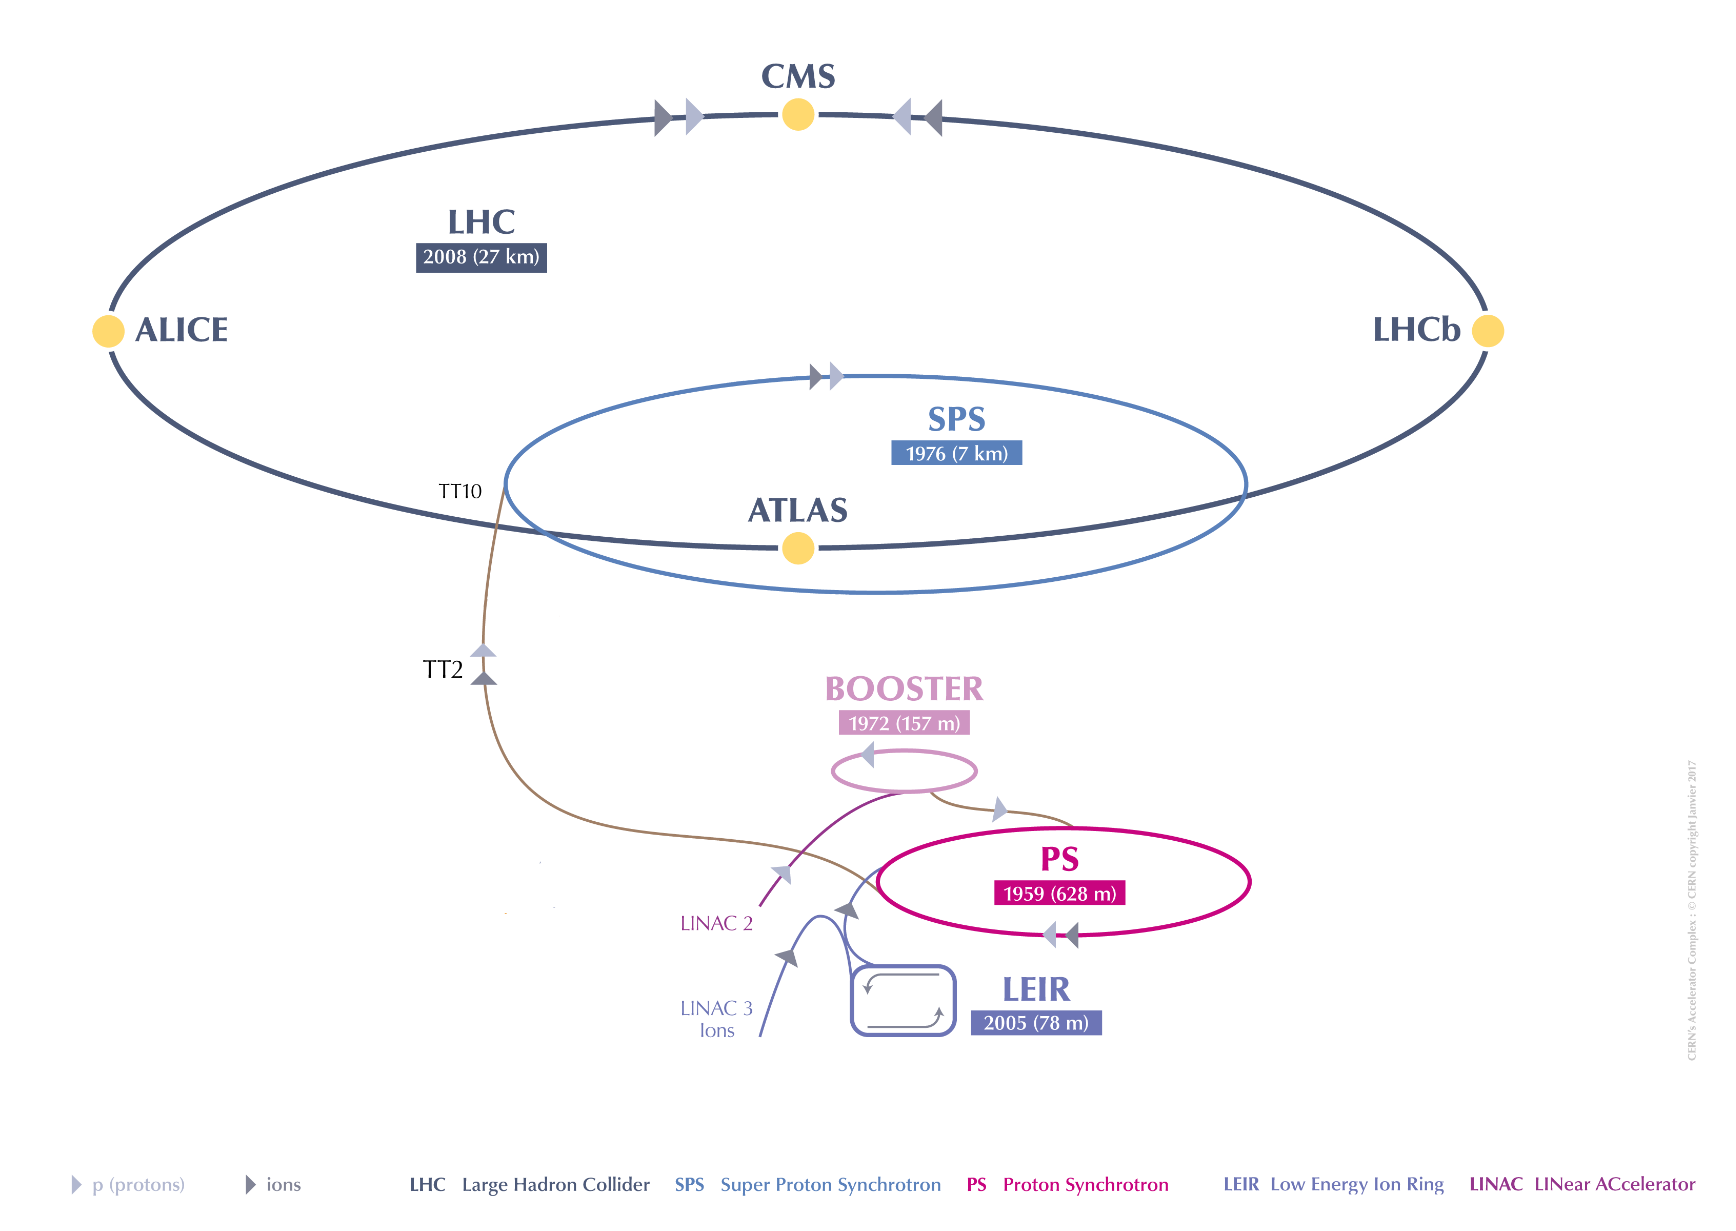
\includegraphics[width=0.95\textwidth]{figures/experiment/cernaccelerators.png}
    \caption{The CERN accelerator complex. The illustration shows the LHC ring and the associated pre-accelerator chain relevant for producing \HepProcess{\Pp\Pp} collisions. Figure adapted from Ref.~\cite{Mobs:2197559}.}
    \label{fig:LHC-chain}
\end{figure}

They start their journey as hydrogen atoms, supplied from a simple gas bottle and ionised by stripping them of their electrons in a duoplasmatron machine~\cite{Bailey2014}.
The protons emerge as a beam with \SI{300}{\milli\ampere} current and are first accelerated to \(\sqrt{s} = \SI{50}{\mega\electronvolt}\) by the LINAC2 linear accelerator.
The Proton Synchroton Booster (PSB) and the Proton Synchrotron (PS) perform the next acceleration stages. Both are synchrotron accelerators. The PSB consists of four synchrotron rings with a radius of \SI{25}{\meter}, which are stacked on top of each other, and accelerates the protons to \(\sqrt{s} = \SI{1.4}{\giga\electronvolt}\). The PS extends over large parts of the CERN Meyrin site with a radius of \SI{100}{\meter} and raises the beam energy to \SI{25}{\giga\electronvolt}. As each of the four PSB rings extends one-quarter of the PS circumference, the PSB beam can be extracted sequentially to the PS. As the beams are extracted and injected by kicker magnets, pulsed dipole magnets with swift time response, they arrive not continuously but in discrete bunches.
The Super Proton Synchrotron, extending \SI{7}{\kilo\meter} in circumference, ramps up the beam energy to \SI{450}{\giga\electronvolt} before the proton beams are injected in the two storage rings of the LHC.

In the LHC, particles are accelerated by radio frequency (RF) cavities driven by high power klystrons. The RF system is operated at \SI{400.79}{\mega\hertz} with each cavity providing a field gradient of \SI{5.5}{\mega\volt\per\meter} and \SI{2}{\mega\electronvolt} acceleration voltage, resulting in a total increase of the beam energy by \SI{485}{\kilo\electronvolt} per revolution.

The LHC beams are kept on their circular trajectories by \num{1232} superconducting niobium-titanium dipole magnets operated at a temperature of \SI{1.9}{\kelvin} with magnetic field strengths of \SI{8.33}{\tesla}. The space constraints imposed by the tunnel require a twin-bore magnet design, hosting the two beam pipes and two sets of magnet coils within the same mechanical structure and cryostat. The beams are focussed using quadrupole and higher-order multipole magnets.

The machine luminosity is determined by several beam parameters, which are listed in \Cref{tab:lhcparameters}, and can be written as
\begin{align}
    L = \frac{N_{b}^2 n_b f_{\text{rev}} \gamma_r F}{4 \pi \varepsilon_n \beta^{*}}.
\end{align}

The luminosity is determined by in-situ measurements performed with dedicated detectors and van-der-Meer scans~\cite{vanderMeer:296752,ATLAS-CONF-2019-021}.

\begin{table}
\caption{Essential LHC parameters with their description and values during Run-2 operation~\cite{Evans2008}.}
\label{tab:lhcparameters}
\resizebox{1.0\textwidth}{!}{%
\begin{tabular}{llr}
\toprule
Parameter & Description & Value \\
\midrule
\(E\) & beam energy & \SI{6.5}{\tera\electronvolt} \\
\(L_{\text{inst}}\)& peak luminosity & \SI{2e34}{\per\square\centi\meter\per\second}\\
\(N_b\) & particles per bunch& \num{1.15e11} \\
\(n_b\) & bunches per beam & \num{2808} \\
\(f_{\text{rev}}\) & revolution frequency & \SI{11.245}{\kilo\hertz} \\
\(\gamma\) & relativistic gamma factor & \num{7461} \\
\(\varepsilon_n\) & normalised transverse beam emittance & \SI{3.75}{\micro\meter}\\
\(\beta^{*}\) & \(\beta\) function at collision point & \SI{0.5}{\meter}\\
\multirow{2}{*}{\(F\)} & geometric luminosity reduction factor & \multirow{2}{*}{\num{0.836}}\\
& due to crossing angle at interaction point & \\
\bottomrule
\end{tabular}}
\end{table}

The two beams intersect at four interaction points, each within a cavern hosting one of the four extensive LHC experiments ATLAS~\cite{ATLAS2008}, LHCb~\cite{LHCB2008}, CMS~\cite{CMS2008}, and ALICE~\cite{ALICE2008}.
In total, there are eight LHC experiments. The three smaller experiments, TOTEM~\cite{TOTEM2008}, LHCf~\cite{LHCF2008}, MoEDAL~\cite{Mitsou2017}, and FASER~\cite{Ariga:2651328}, complement the LHC physics programme by more specific measurements. TOTEM and LHCf use detectors positioned close to the CMS and ATLAS experiment, respectively, to investigate the physics of particles generated almost directly in line with the colliding proton beams. The prime goal of the MoEDAL experiment, which shares the cavern with LHCb, is the search for magnetic monopoles and exotic particles.
The FASER experiment, which is located in a service tunnel downstream from the interaction point used by the ATLAS experiment, searches for light, weakly-coupled particles and investigates the interactions of high-energy neutrinos.
The LHCb experiment is a specialised detector investigating flavour physics. The ALICE experiment investigates physics of strongly interacting matter at extreme energy densities by analysing heavy lead ion collisions. The two all-purpose detectors ATLAS and CMS, operated at peak luminosity, are located in opposed caverns. Their independent operation and different detector design are crucial for cross-checks and reciprocal corroboration in the event of a potential discovery.

Although high beam intensities enhance searches for rare processes by increasing the collected data over time, they also increase the number of simultaneous \HepProcess{\Pp\Pp} interactions in a single collision event. Such multiple \HepProcess{\Pp\Pp} interactions are known as pile-up and are typically uncorrelated with the hard-scattering process. Therefore, they contribute a largely diffuse background of primarily soft energy depositions in the detector. One distinguishes between in-time pile-up, which refers to multiple collision events within the same bunch crossing, and out-of-time-pileup, which refers to energy deposits from previous and following bunch crossings concerning the triggered event. The total expected amount of pile-up \(\mu\) is related to the instantaneous luminosity by the equation
\begin{align}
    \mu = \frac{\mathcal{L} \sigma_{\text{inel}}}{N_b n_b f_{\text{rev}}},
\end{align}
where \(\sigma_{\text{inel}} = \SI{78.1 \pm 2.9}{\milli\barn}\) is the inelastic \HepProcess{\Pp\Pp} cross-section~\cite{STDM-2015-05}.


\section{The ATLAS detector}
\label{sec:experiment:ATLAS}
The ATLAS detector is a multi-purpose detector for recording collisions at the LHC. Its design is influenced by both the extreme conditions at the LHC and by the requirements for precision measurements and potential discovery of new physics processes at the \si{\tera\electronvolt} scale.
The high interaction rates and radiation doses delivered to LHC detectors require fast, radiation-hard electronics and detector elements with high granularity. The demands for performing high precision tests of quantum chromodynamics,  exploring the mechanism of electroweak symmetry breaking, and searching for signatures of new physics phenomena dictate the design of the detector and its subsystems.

The ATLAS detector has a cylindrical geometry and extends \SI{44}{\meter} in length and \SI{25}{\meter} in diameter with a weight of \SI{7000}{\tonne}. A sketch of the ATLAS detector, highlighting its various subsystems, is provided in \Cref{fig:ATLAS-full}.

\begin{figure*}[htbp]
    \centering
    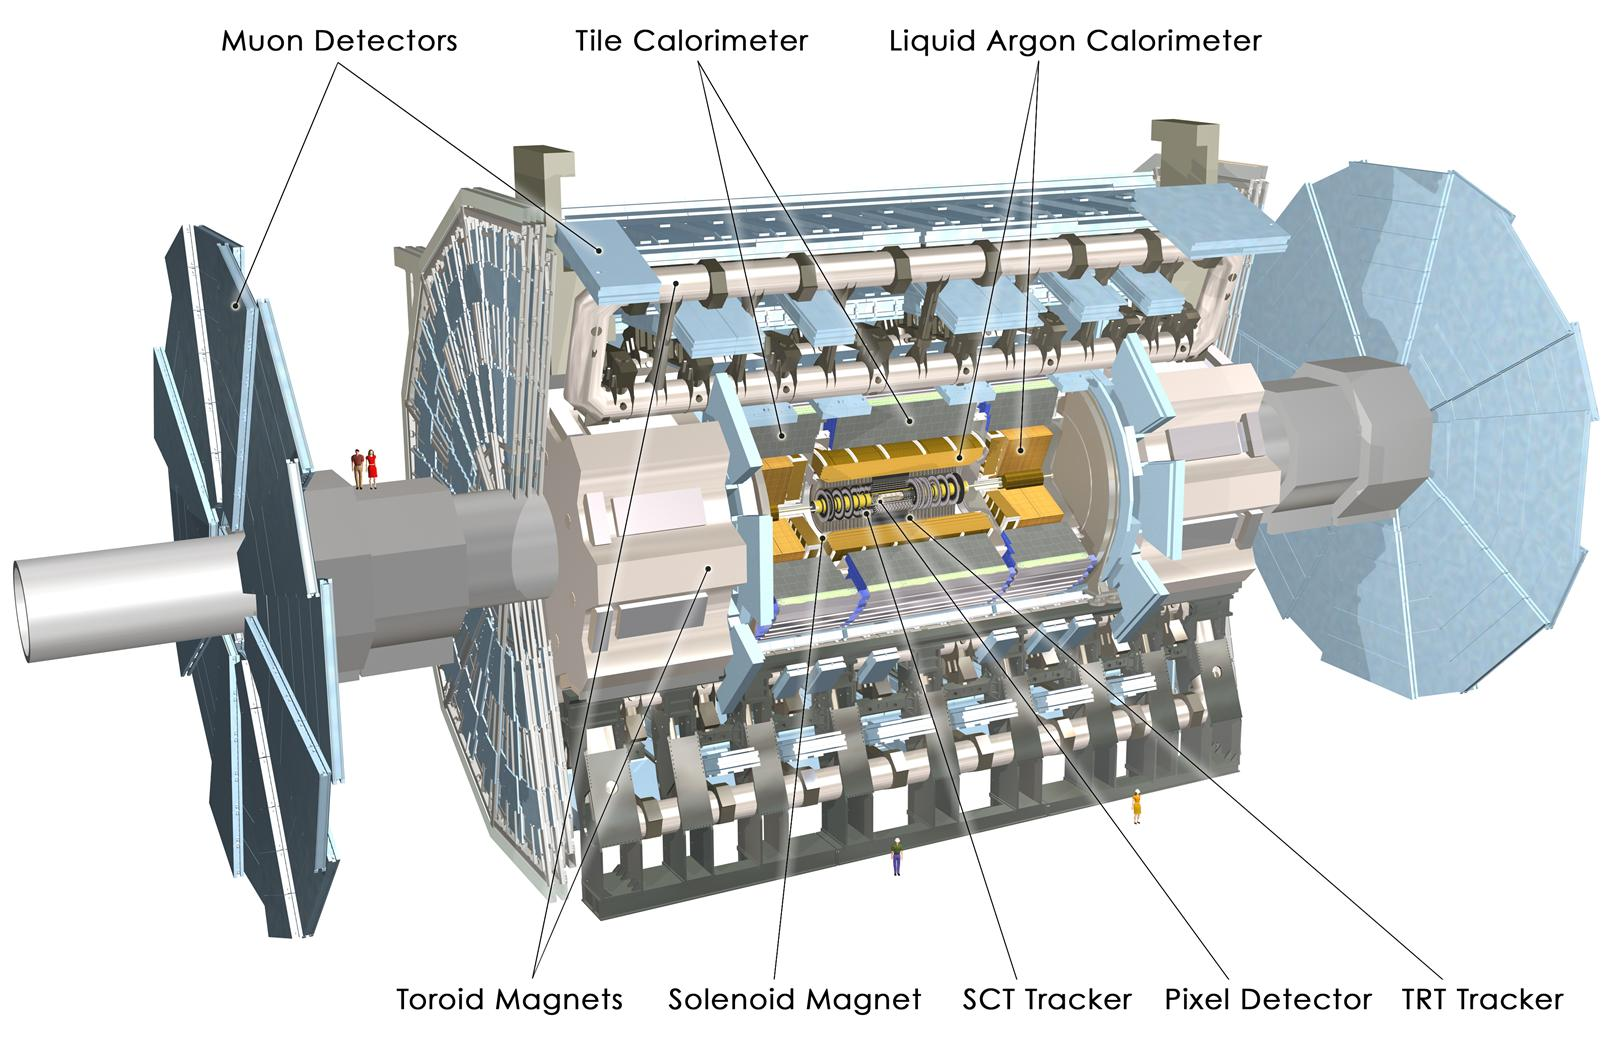
\includegraphics[width=0.95\textwidth]{figures/experiment/detector_full.jpg}
    \caption{Schematic representation of the ATLAS detector and its various subsystems. Figure reproduced from Ref.~\cite{ATLAS2008}.}
    \label{fig:ATLAS-full}
\end{figure*}

The detector consists of a cylindrical barrel region and two wheel-shaped end-caps, each instrumented with detector subsystems to achieve full coverage in the full \(4\pi\) solid angle. The detector geometry possesses an eightfold symmetry around the beam axis and a forward-backwards symmetry to the interaction point.
The detector is comprised of three main subsystems, starting with the innermost component, the inner detector, calorimeters and muon spectrometer. They are introduced briefly in the following. A detailed description of the ATLAS detector is provided in Ref.~\cite{ATLAS2008}.
\subsection{The ATLAS coordinate system}
The ATLAS coordinate system is used throughout this dissertation and defined by expressing space-time events in terms of a right-handed Cartesian coordinate system with its origin located at the nominal interaction point.
The \(z\)-axis is defined by the beam axis, the positive \(x\)-axis points from the interaction point to the centre of the LHC ring, and the positive \(y\)-axis points towards the earth's surface.
The symmetry of the experiment favours a cylindrical coordinate system with the azimuthal angle \(\varphi\) measured around the beam axis and the polar angle \(\theta\) measured from the beam axis.
In collider experiments, it is common practice to express the inclination of a particle with four-momentum \(p = (E, \vec{p})\) to the beam with the pseudorapidity
\begin{align}
    \eta = - \ln \tan{\frac{\theta}{2}} = \frac{1}{2} \cdot \ln{\frac{\abs{\vec{p}} + p_z}{\abs{\vec{p}} - p_z}}.
\end{align}
The pseudorapidity is zero in transverse direction and increases rapidly for smaller inclinations with respect to the beam axis.
In the relativistic limit, the pseudorapidity approaches to the rapidity
\begin{align}
    y = \frac{1}{2} \cdot \ln{\frac{E + p_z}{E - p_z}}.
\end{align}
The phase-space measure of a particle \(\dd{\Pi}_{f}\) is proportional to the rapidity, thus the particle flux per rapidity interval is approximately constant.
Differences in rapidity (and by extension also the pseudorapidity) are invariants under Lorentz boosts along the beams axis. As a consequence, measurements of rapidity differences \(\Delta y\) between particles are the same in different reference frames connected by a Lorentz boost along the beam axis. An invariant distance measure can be defined in the pseudorapidity-azimuthal angle space as
\begin{align}
    \Delta R = \sqrt{\Delta \eta^2 + \Delta \varphi^2} = \sqrt{(\eta_1 - \eta_2)^2 + (\varphi_1 - \varphi_2)^2}.
\end{align}
The composite nature of the colliding protons only allows specifying the transverse momentum component of initial state partons taking part in the hard-scattering process. The aforementioned property of the rapidity therefore is crucially important for interpreting measurements of particles created in \HepProcess{\Pp\Pp} collisions. In a similar vein, it is useful to define transverse quantities of observables, such the transverse momentum
\begin{align}
    p_{\text{T}} = \abs{\vec{p}} \sin{\theta} = \abs{\vec{p}} \cosh{\eta}
\end{align}
which is the projection of the momentum \(p\) onto the \(x\)-\(y\) plane.
Similarly, the missing transverse momentum component in the \(x\)-\(y\) plane \(E_{\text{T}}^{\text{miss}}\) is of particular importance for dark matter searches.
Other variables to describe the trajectory of a particle are the transverse impact parameter \(d_0\) and the longitudinal impact parameter \(z_0\). These are defined as the closest distance between the particle's trajectory and the reconstructed primary vertex in the transverse plane or longitudinal \(z\)-direction, respectively.


\subsection{Magnet system}
\label{sec:experiment:ATLAS:magnets}
Momentum and charge measurement of charged particles requires the bending of their trajectories by being immersed in magnetic fields. To this end, ATLAS is equipped with a magnet system consisting of four large superconducting magnets. All magnets employ superconducting niobium-titanium technology and are cooled to about \SI{4.5}{\kelvin} using liquid helium-3. The energy stored in the ATLAS magnets during operation amounts to \SI{1.6}{\giga\joule}.
The central solenoid magnet is aligned on the beam pipe and provides a \SI{2}{\tesla} axial magnetic field for charged particle measurements in the inner detector. It extends over \SI{5.3}{\meter} length and has a diameter of \SI{2.5}{\meter}. As the magnet is situated between tracking and calorimetry system, a large material budget would impact the calorimeter resolution. The solenoid assembly contributes roughly \num{0.66} radiation lengths at normal incidence, realised by an extremely light-weight structure and shared cooling elements of the solenoid and the calorimeter system.
The barrel toroid and two end-cap toroids are defining for the ATLAS experiment as they not define the name of the experiment but also shape the total dimensions of the detector. The barrel toroid consists of eight air-core race-track shaped coils with an overall length of \SI{25.3}{\meter} covering the region in between \SIrange{9.4}{20.1}{\meter} from the interaction region.
The end-cap toroids are octagonal wheels equipped with eight flat, square toroidal coil units and eight keystone wedges.
Together, the toroids provide toroidal magnetic fields of approximately \SI{0.5}{\tesla} and \SI{1.0}{\tesla} for the muon detectors in the central and the end-cap regions, respectively. The highly non-uniform toroidal field requires a high-precision field mapping by approximately \num{1800} Hall sensors distributed throughout the spectrometer volume.

\subsection{Inner Detector}
\label{sec:ATLAS-ID}
The inner detector provides precision measurements of charged particle trajectories. As it is immersed in the \SI{2}{\tesla} solenoid magnetic field, the track curvature can be used for determining the track's transverse momentum \(p_{\text{T}}\).
The reconstructed particle tracks are used for pattern recognition to identify common points of origin, which are called vertices. The primary vertex is the vertex with the highest scalar \(p_{\text{T}}\) sum of associated tracks satisfying transverse and longitudinal impact parameter requirements. The primary vertex corresponds to the hardest interaction in the event, which typically is the interaction of interest. Other vertices in the same bunch crossing can be used to identify signatures associated with pile-up. Additionally, secondary vertices, which correspond to the displaced decays of short-lived particles, are used to identify the production of \(b\)-quarks or \(\tau\) leptons.
To this end, the inner detector is located close to the interaction region. It is comprised of discrete, high-resolution semiconductor pixel and strip detectors in the inner part of the tracking volume and straw tube tracking detectors in the outer part, with additional capability for particle identification by generating and detecting transition radiation. An essential design requirement is a light material budget to reduce energy losses in the ID.
The momentum resolution of the inner tracker for trajectories of particles with transverse momentum \(p_{\text{T}}\)is approximately
\begin{align}
    \frac{\sigma(p_{\text{T}})}{p_{\text{T}}} = \sqrt{\left(0.05 \% \cdot \left(\frac{p_{\text{T}}}{\si{\giga\electronvolt}}\right)\right)^2 + \left(1 \%\right)^2}.
\end{align}
The layout of the inner detector is illustrated in \Cref{fig:innerdetector}.

\begin{figure}[htbp]
\begin{subfigure}{1.\textwidth}
  \centering
  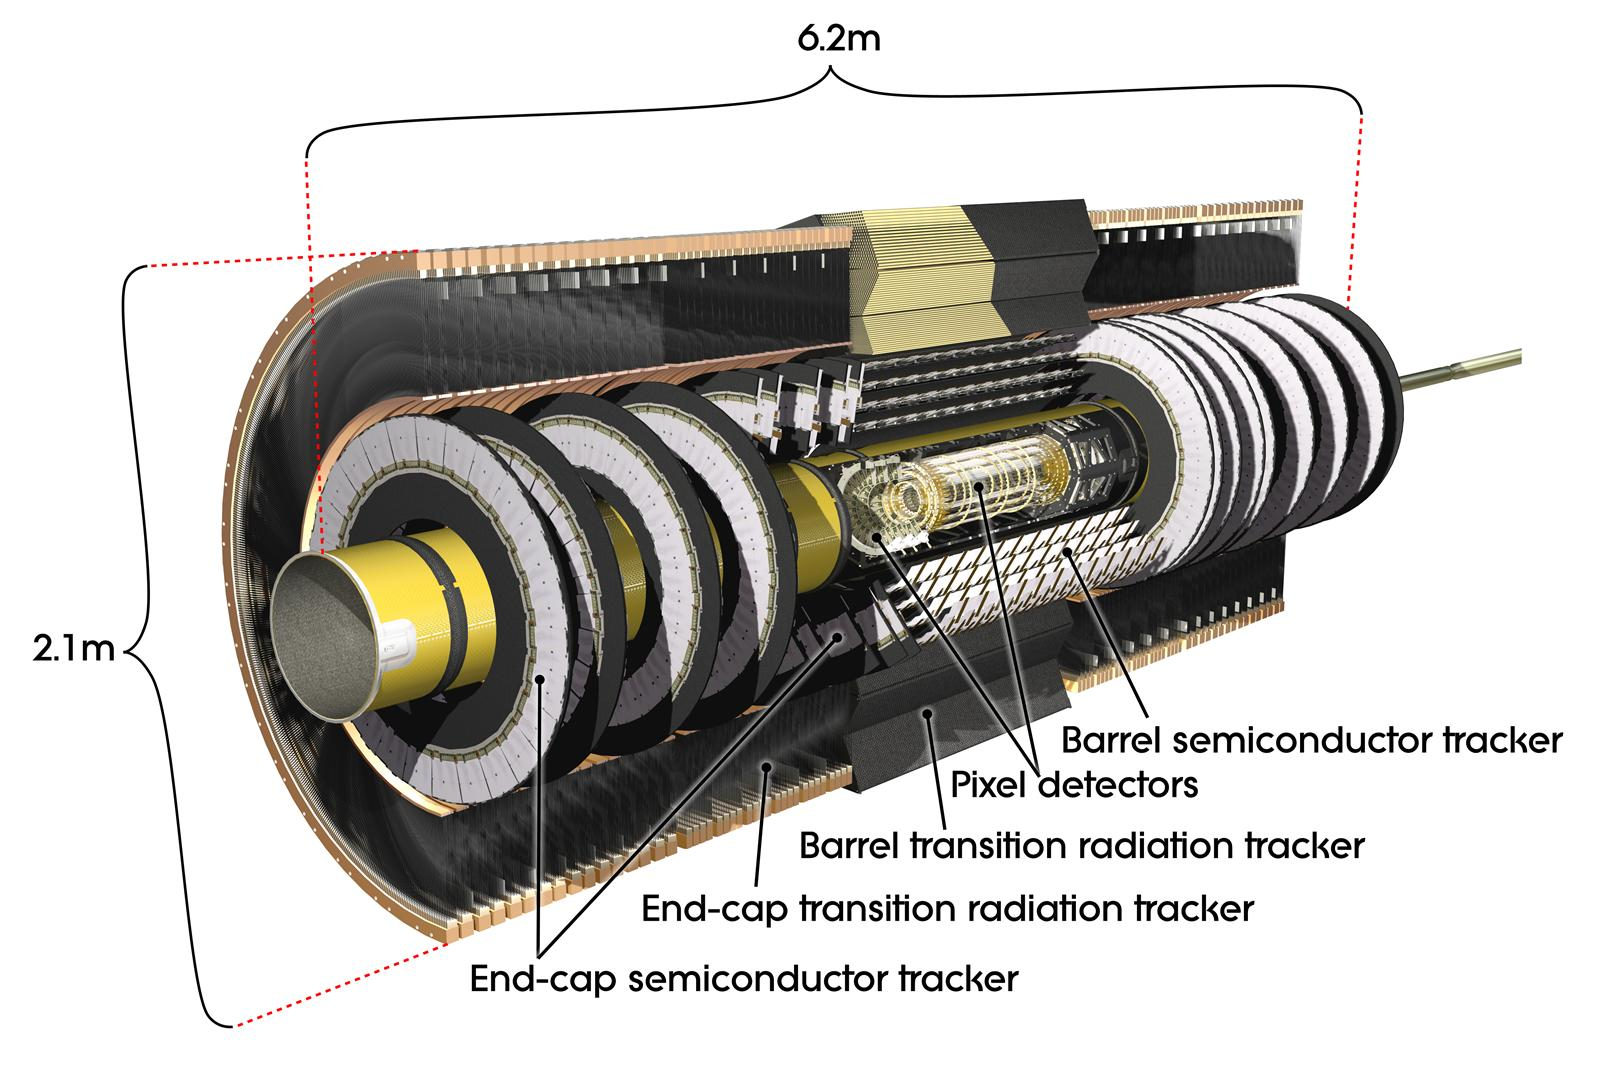
\includegraphics[width=0.95\textwidth]{figures/experiment/innerdetector_full.jpg}
  \caption{Overview of the ID and its sub-detectors. Figure reproduced from Ref.~\cite{ATLAS2008}.}
  \label{fig:innerdetector-full}
\end{subfigure}
\\
\begin{subfigure}{1.\textwidth}
  \centering
  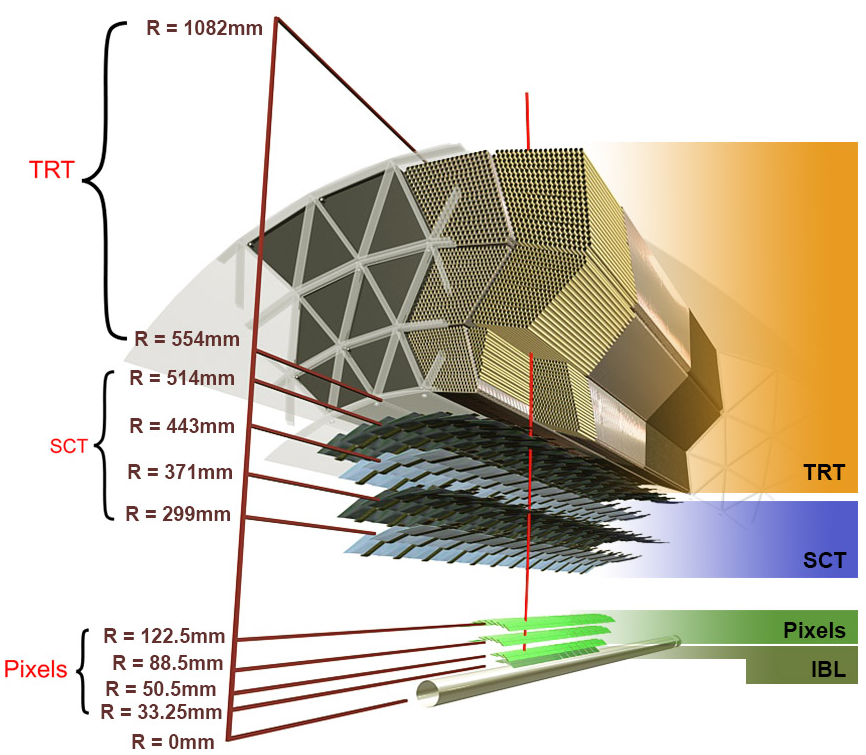
\includegraphics[width=.95\textwidth]{figures/experiment/innerdetector_detail.png}
  \caption{Detailed layout of the ID traversed by a charged track in the barrel region at \(\eta = 0.3\). The track traverses the beam pipe, the four cylindrical PXD layers, the four SCT layers, and approximately 36 axial straws contained within the TRT modules. Figure reproduced from Ref.~\cite{Potamianos:2016ptf}.}
  \label{fig:innerdetector-detail}
\end{subfigure}
    \caption{Illustrations of the ID layout and its spatial dimensions.}
    \label{fig:innerdetector}
\end{figure}

The silicon pixel detector (PXD) is located closest to the beam axis in \SI{12}{\centi\meter} radial distance. Four layers of silicon pixel modules with \num{8.4e7} readout channels provide accurate three-dimensional information with the highest granularity.
In the barrel region, the detector modules are arranged on four concentric cylinders around the beam axis positioned at radii of \SI{33.25}{\milli\meter}, \SI{50.5}{\milli\meter}, \SI{88.5}{\milli\meter}, and \SI{122.5}{\milli\meter}, while in the end-cap regions they are located on six disks perpendicular to the beam axis at distances \(\pm\SI{495}{\milli\meter}\), \(\pm\SI{580}{\milli\meter}\), and \(\pm\SI{650}{\milli\meter}\) from the collision point.
The innermost barrel module, the insertable \(b\)-layer (IBL)~\cite{Abbott2018,CERN-LHCC-2010-013,CERN-LHCC-2012-009}, substantially contributes to the high precision impact parameter measurements, which are critical for vertex identification, by its proximity to the beamline and high spatial resolution.
The PXD provides typically four measurement points for charged particles originating in the beam-interaction region with \SI{10}{\micro\meter} spatial resolution in the transverse plane and \SI{115}{\micro\meter} in the longitudinal \(z\)-direction.

The silicon microstrip tracker (SCT) forms the middle layer of the ID and extends up to \SI{52}{\centi\meter} in the radial distance. As it is located further away from the beamline than the PXD, coarser granularity achieved by \num{6.3e6} readout channels is sufficient. It consists of four concentric layers of silicon strip detectors in the barrel region and 18 wheel-shaped disks containing the sensor modules in the end-cap regions.
Each module hosts two single-sided silicon micros-trip sensor plates rotated about a stereo angle of \SI{40}{\milli\radian} to enable two-dimensional position measurements.
The two precision semiconductor tracking detectors cover the region \(\abs{\eta} < 2.5\). They are connected to a cooling system to reduce noise after irradiation. Their alignment is monitored by comparing positions of module hits with intersections of reconstructed tracks with the modules. Additionally, the SCT alignment is monitored by an interferometry system.
The SCT provides typically eight hits per track at intermediate radii with \SI{17}{\micro\meter} spatial resolution in the transverse plane and \SI{580}{\micro\meter} in the longitudinal \(z\)-direction.

The transition radiation tube tracker (TRT) constitutes the outermost layer of the ID and operates with \num{3.4e5} readout channels. The TRT employs proportional drift tube arrays made of polyimide for track measurements. The choice of drift tubes as detector technology not only allows for the instrumentation of a large volume at comparably low cost but also avoids cooling issues and supports maintaining a low material budget for the ID.
The tubes with diameter of \SI{4}{\milli\meter} contain a \SI{30}{\micro\meter} gold-plated tungsten wire in their centre and are filled with a (\SI{70}{\percent} \ch{Xe} / \SI{27}{\percent} \ch{CO2} / \SI{3}{\percent} \ch{O2}) gas mixture\footnote{As gas leaks occurred during operation of the TRT, some of the TRT modules instead contain an \ch{Ar}-based gas mixture. The presence of this gas mixture is taken into account in the simulation, and the reduced efficiency of \ch{Ar} is partially mitigated by dedicated reconstruction algorithms.}. The tubes are kept at the negative voltage of \SI{1530}{\volt} with their wire kept at ground. The resulting electric field accelerates particles traversing the tubes, which then ionise the gas mixture. As a result, the ionisation products drift to the respective electrode of opposite polarity. Near the wire anode, the field strength is sufficiently high for the electron to create an avalanche of new ionisation processes, manifesting in a signal proportional to the number of primary charges. This measurement determines the primary electron drift time. Based on the knowledge of the drift velocity of electrons in the gas mixture, the radius of the closest approach between the particle trajectory and the wire can be computed. Combining measurements from several individual drift tubes allows determining the particle trajectory unambiguously.
The TRT covers the region \(\abs{\eta} < 2.0\). It provides typically \num{35} hits per track with \(p_{\text{T}} > \SI{0.5}{\giga\electronvolt}\) with \SI{130}{\micro\meter} spatial resolution in the plane orthogonal to the drift tubes.

\subsection{Calorimetry}
\label{sec:experiment:ATLAS:calorimetry}
The ATLAS calorimeter can identify electrons, photons, and hadrons and provides measurements of their energy and position.
The principle underpinning calorimetry is the destructive energy measurement of incoming particles by a chain of inelastic reactions leading to a shower of secondary particles, which in turn deposit their energy to active detector material. There, a fraction of the energy is converted into measurable quantities, which can be related to the total absorbed energy by a calibration procedure. Position measurements with coarse resolution can be achieved by segmenting the calorimeter into individual cells.
Electromagnetically and hadronically interacting particles have different mechanisms for shower formation. The energy loss of electrons happens mostly via bremsstrahlung, whereas the dominant process for photons is pair production. The interplay of both processes results in the electromagnetic shower. The characteristic length scale for both processes is the radiation length \(X_0\), defined as the distance over which an electron radiates off \SI{63}{\percent} of its energy.
The interactions of hadrons are more complex and involve a cascade of inelastic hadronic interactions. The characteristic length scale for hadronic interactions with matter is the interaction length \(\lambda\), which is defined as the mean distance travelled by a hadronic particle before undergoing an inelastic nuclear interaction.
Two particular types of calorimeters are encountered in collider experiments. Electromagnetic calorimeters typically employ inorganic crystals or liquid noble gases with high nuclear charge \(Z\) as the active material. Hadronic calorimeters typically layer the active material with very dense material, such as iron, to stop the hadronic showers, whose depth of penetration into the calorimeter exceeds that of electromagnetic showers.

Calorimetry complements the tracking detectors in two ways.
\begin{enumerate}
    \item The energy resolution of calorimeters increases for larger energy \(\sigma(E) / E \propto 1 / \sqrt{E}\) due to the Poisson statistics of the shower, whereas the resolution of curvature-based momentum measurements deteriorates for larger momenta, following the relation \(\sigma(p) / p \propto p\).
    \item Calorimeters are sensitive to both charged and neutral particles. As the emergent parton shower due to hadronic final states, which are at the focus of this dissertation, is a mixture of both neutral and charged particles, calorimeters are essential for their accurate measurement.
\end{enumerate}

An overview of the ATLAS calorimetry system is given in \Cref{fig:calorimetry-full}.
\begin{figure}[htbp]
    \centering
    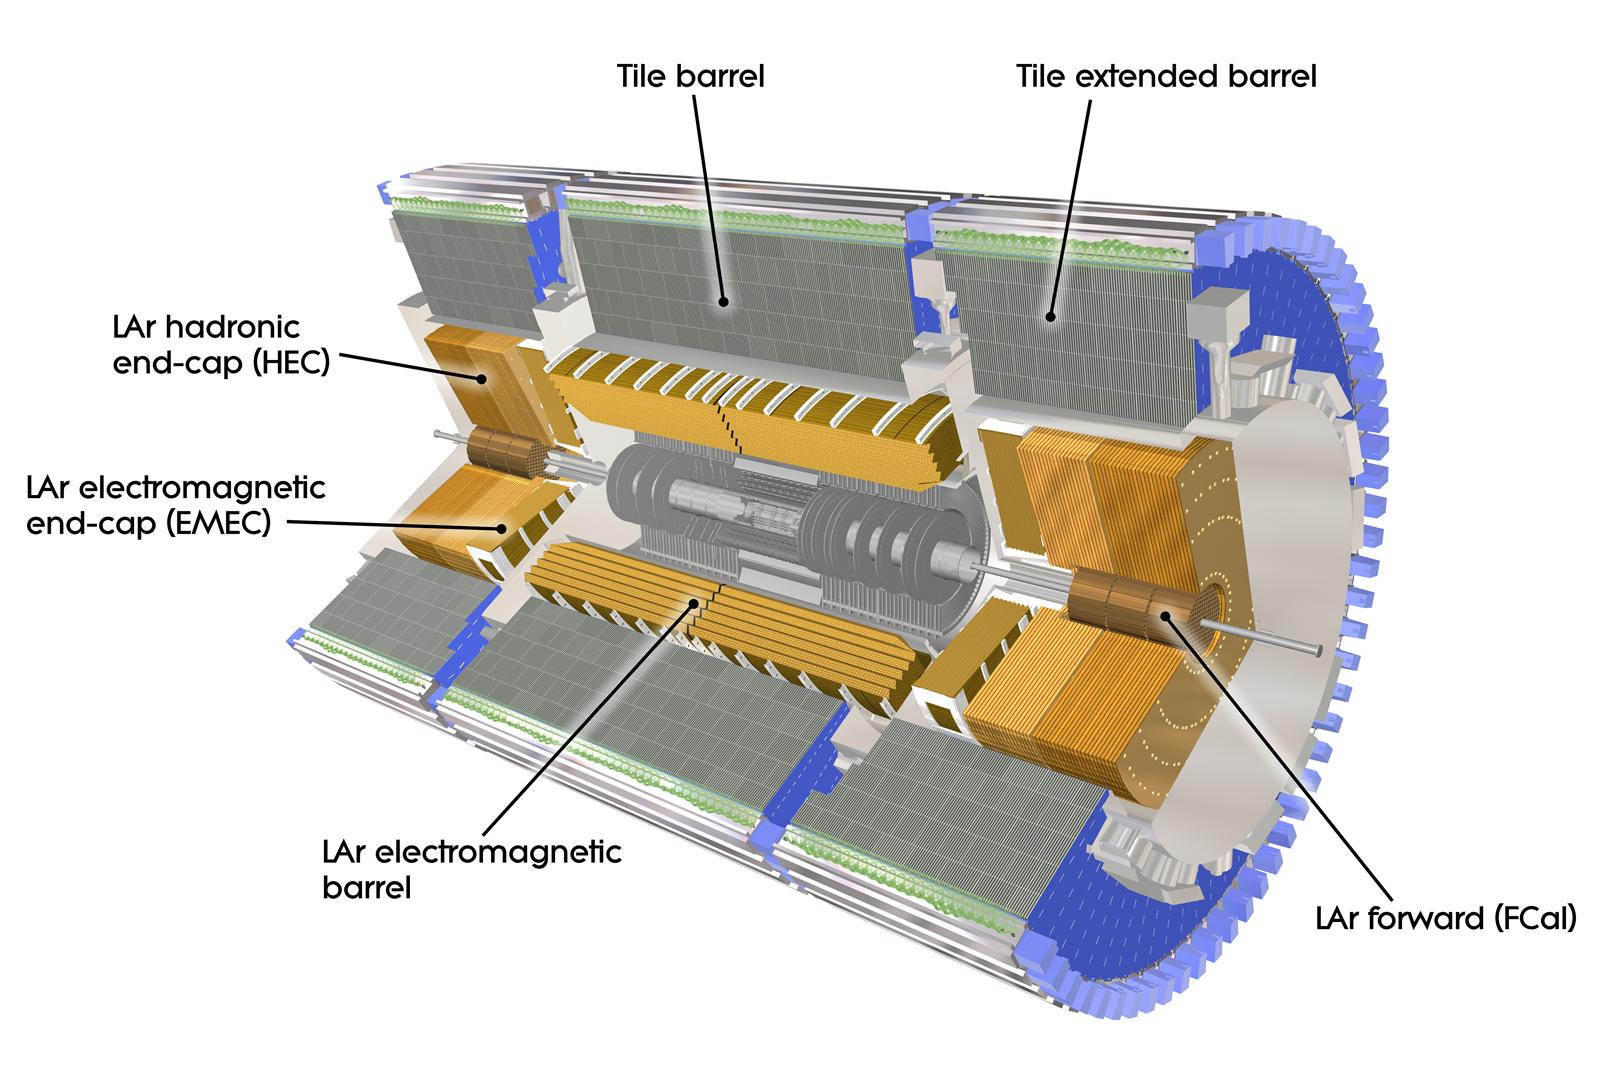
\includegraphics[width=0.95\textwidth]{figures/experiment/calorimetry_full.jpg}
    \caption{The ATLAS calorimeter system with its various components. Figure reproduced from Ref.~\cite{ATLAS2008}.}
    \label{fig:calorimetry-full}
\end{figure}

The ATLAS calorimeter system surrounds both the ID and the solenoid. It has a length of \SI{12.2}{\meter} and extends to an outer radius of \SI{4.25}{\meter}. Its geometry is fully symmetric in \(\varphi\) and has full coverage around the beam axis and covers the pseudorapidity range \(\abs{\eta} < 4.9\). The enormous energy of particles created in LHC \HepProcess{\Pp\Pp} collisions necessitates shortening of the absorption length by the use of calorimeters with alternating layers of active detector material and passive, purely absorbing material. This sampling calorimeter design is used in all ATLAS calorimeters.
The calorimeter system is comprised of electromagnetic calorimeters in the barrel and end-cap regions, enclosed by the hadronic calorimeters and complemented by dedicated calorimeters in the forward region close to the beam pipe. The ATLAS calorimeter system is hosted in three cryostats. The barrel cryostat contains the central solenoid and the electromagnetic barrel calorimeter. The end-cap cryostats each contain one electromagnetic end-cap calorimeter, one hadronic end-cap calorimeter, and one forward calorimeter.
The design of the calorimetry system ensures full containment of electromagnetic and hadronic showers and reduction of punch-through into the muon spectrometer. The electromagnetic calorimeters have more than \num{22} radiation lengths \(X_0\) in the barrel region and more than \num{24} radiation lengths in the end-cap regions. The hadronic calorimeters have an interaction length \(\lambda\) of approximately \num{9.8} in the barrel region and an interaction length of about \num{10} in the end-cap region. The forward calorimeter has an interaction length \(\lambda\) of approximately \num{10}.

The electromagnetic calorimeters cover the pseudorapidity range \(\abs{\eta} < 3.2\). The active detector medium is radiation hard Liquid Argon (LAr), which is chosen for its stability and linear response. The passive layers are made of lead. The absorber plates are shaped in an accordion geometry, thus providing full coverage in \(\varphi\) without cracks.
The barrel electromagnetic calorimeter covers the pseudorapidity range \(0 < \abs{\eta} < 1.475\). It consists of two identical components separated by a \SI{4}{\milli\meter} gap at \(\eta = 0\).
The two end-cap electromagnetic calorimeters (EMEC) cover the pseudorapidity range \(1.375 < \abs{\eta} < 3.2\). They consist each of two coaxial wheels with a small non-overlapping region at \(\abs{\eta} = 2.5\).
The transition region between the barrel and the end-cap (\(1.37 < \abs{\eta} < 1.52\)) contains a relatively large amount of inactive material.
In the precision physics region \(\abs{\eta} < 2.47\), where tracking information is available, the electromagnetic calorimeters are segmented in three layers with different granularity to allow for measurements of the electromagnetic shower profile.
The first layer is finely segmented in strips to allow for excellent discrimination between photons from the hard interaction and photons from \Pgpz decays. Most of the electron and photon energy is collected in the second layer, while the third layer measures the energy deposits due to the shower's tails.
The remaining acceptance is segmented in two layers with uniform granularity \(\Delta \phi \times \Delta \eta = 0.1 \times 0.1\).
The energy measurement in the region \(\abs{\eta} < 1.8\) is corrected for the energy loss of particles before entering the calorimeter by the use of two pre-sampling detectors, made of a thin LAr layer.
The combined electromagnetic calorimeter energy resolution is
\begin{align}
    \frac{\sigma_{E}}{E} = \frac{\SI{10}{\percent}}{\sqrt{E}} \oplus \SI{0.7}{\percent},
    \label{eq:experiment:ATLAS:calorimetry:resolution}
\end{align}
where \(\oplus\) indicates the quadratic sum.

The hadronic calorimeter encloses the electromagnetic calorimeters, as the depth of hadronic showers typically exceeds that of electromagnetic showers. Two different calorimeter technologies are employed to address the increasing irradiation in regions closer to the beam pipe.
The pseudorapidity range \(\abs{\eta} < 1.7\) is instrumented with a tile calorimeter, subdivided in a barrel region enclosing the electromagnetic barrel calorimeter and two extended barrel regions, which surround the end-cap calorimeters.
The barrel region covers \(\abs{\eta} < 1.0\) and the two extended barrel regions cover \(0.8 < \abs{\eta} < 1.7\).
Scintillator tiles are used as the active detector medium, while steel is used as the absorber medium.
The tile calorimeter extends \SIrange{2.28}{4.25}{\meter} in the radial direction. Each barrel region is azimuthally divided into 64 modules, corresponding to \(\Delta \varphi = 0.1\), and is segmented into three layers.
The scintillating tiles are read out by wavelength shifting fibres, which are grouped into photomultiplier tubes.
The tile calorimeter provides measurements with an energy resolution of \(\frac{\sigma_{E}}{E} = \frac{50\%}{\sqrt{E}}\).
The pseudorapidity range \(1.5 < \abs{\eta} < 3.2\)%
\footnote{The HEC is overlapping with both the tile calorimeter and the FCal to reduce drops in material density in the transition regions between the calorimeters.} %
is instrumented with a LAr hadron end-cap calorimeter (HEC). It consists of two cylindrical wheels per end-cap, both extending \SI{2.03}{\meter} in the radial direction and hosting each 32 identical wedge-shaped modules. Each wheel is longitudinally divided into two regions of depth and composed from copper plates interspersed with \SI{8.5}{\milli\meter} LAr gaps.
The combined hadronic calorimeter energy resolution for hadronic jets for tile and end-cap calorimeters is
\begin{align}
    \frac{\sigma_{E}}{E} = \frac{\SI{50}{\percent}}{\sqrt{E}} \oplus \SI{3}{\percent}.
\end{align}
The forward region is instrumented with a LAr forward calorimeter (FCal). It covers the pseudorapidity range \(3.1 < \abs{\eta} < 4.9\), thereby ensuring an almost hermetic coverage of the calorimetry system around the interaction point, which is essential for dark matter searches. The FCal consists of three modules in each end-cap, with the first made of copper targeting electromagnetic showers and the remaining two made of tungsten targeting hadronic interactions.
The forward region hadronic calorimeter has an energy resolution for hadronic jets of
\begin{align}
    \frac{\sigma_{E}}{E} = \frac{\SI{100}{\percent}}{\sqrt{E}} \oplus \SI{10}{\percent}.
\end{align}


\subsection{Muon Spectrometer}
\label{sec:experiment:ATLAS:muons}
As muons are substantially heavier than electrons, they do not lose energy by bremsstrahlung and leave only a track footprint because of ionisation energy loss in the calorimeter. Consequently, the particles emerging from the calorimeters are considered to be muons and are detected by a dedicated detector system. The muon spectrometer provides measurements of charged particles exiting the calorimeters, covering the pseudorapidity range \(\abs{\eta} < 2.7\).
It is also able to provide track information in coarser granularity but with timing resolution within a few tens of a nanosecond for the sake of triggering or bunch crossing identification in the pseudorapidity range \(\abs{\eta} < 2.4\). To this end, the muon spectrometer is equipped with sets of precision tracking detectors and trigger chambers. The magnetic field provided by the toroid magnets allows measuring the muon momentum based on the sagitta of the curved trajectory. The detector resolution is optimised for measurements in the plane in the principal bending direction, the so-called bending plane. The layout of the ATLAS muon spectrometer is shown in \Cref{fig:muonspectrometer-full}.

\begin{figure}[htbp]
    \centering
    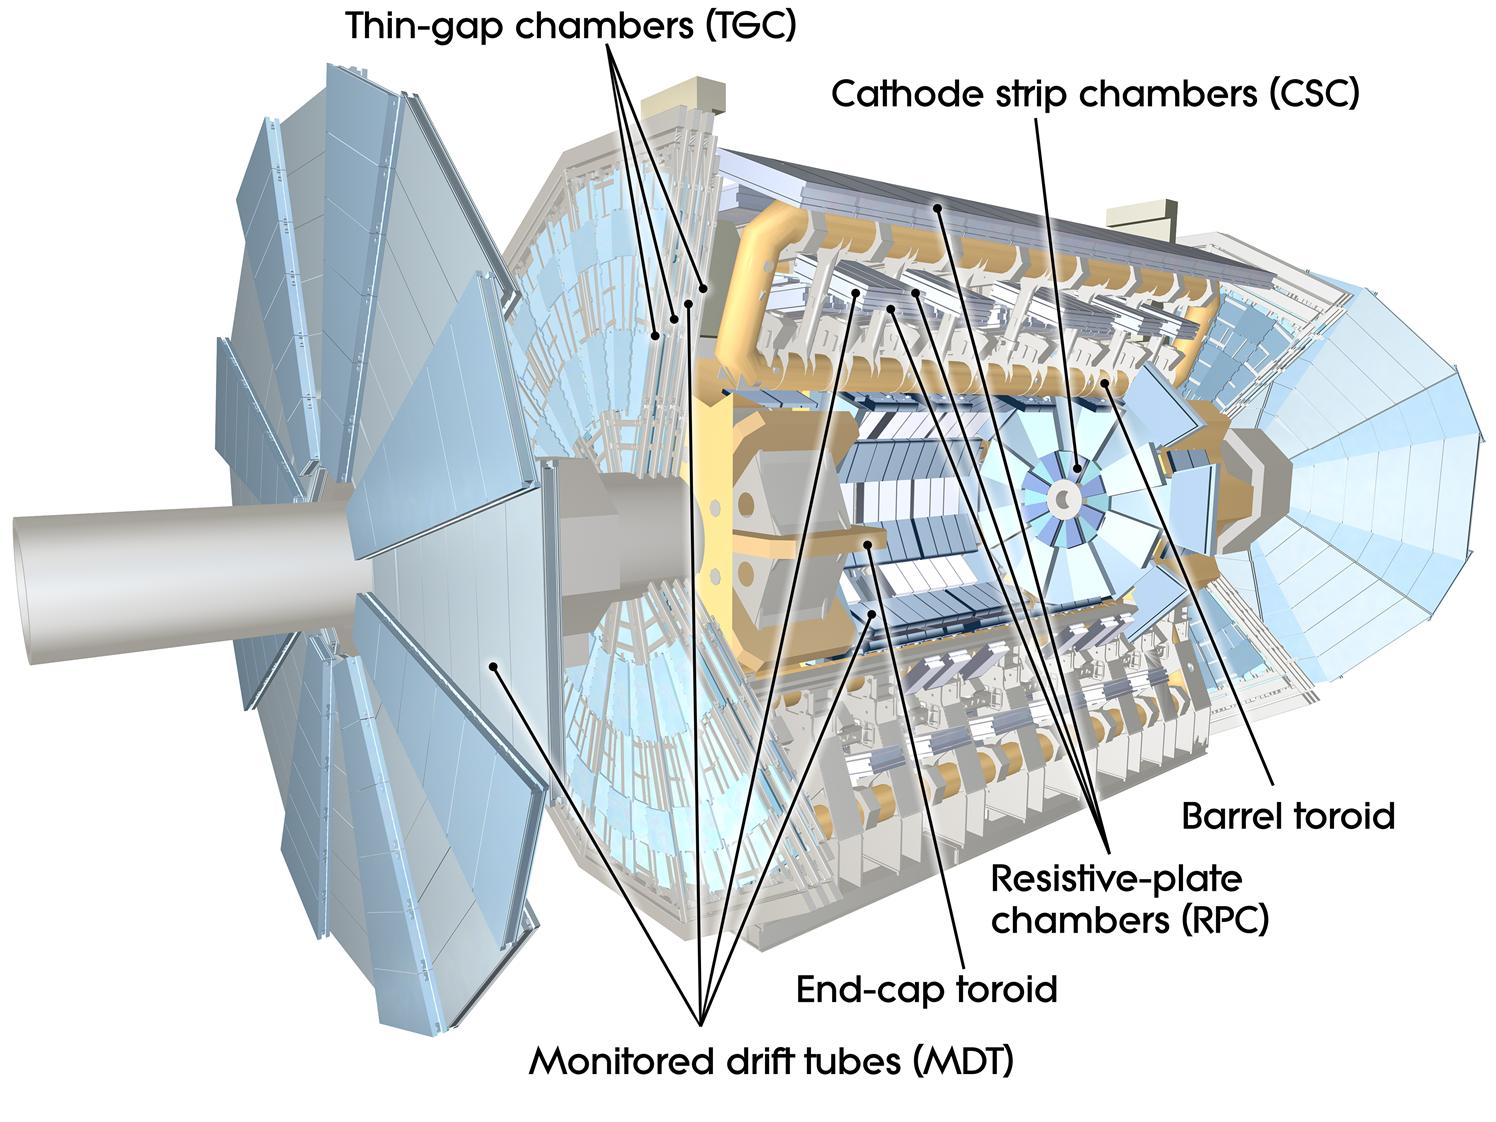
\includegraphics[width=0.95\textwidth]{figures/experiment/muonspectrometer_full.jpg}
    \caption{The ATLAS muon spectrometer with its various components. Figure reproduced from Ref.~\cite{ATLAS2008}.}
    \label{fig:muonspectrometer-full}
\end{figure}

The \num{1150} monitored drift tube (MDT) chambers, whose length and shape depends on their position in the detector, perform the precision measurements.
In the barrel region, they are located between and on the toroid coils. The symmetry of the toroid magnet is reflected in the muon system's geometry, which is divided into octants.
Each octant is subdivided in the azimuthal direction into a large and small sector. The overlap between the different sector types minimises gaps in acceptance and allows for relative alignment of adjacent sectors using tracks measured in both sectors. The chambers in the barrel region are arranged in three concentric cylindrical shells, located at \SI{5}{\meter}, \SI{7.5}{\meter}, and \SI{10}{\meter} in the radial distance to the beam axis.
In the end-cap region the MDT chambers form four large wheels perpendicular to the \(z\)-axis, which are located in front and behind the end-cap toroid magnet. They are located at distances of \(\abs{z}=\SI{7.4}{\meter}\), \(\abs{z}=\SI{10.8}{\meter}\), \(\abs{z}=\SI{14}{\meter}\), and \(\abs{z}=\SI{21.5}{\meter}\) to the interaction point.
An MDT chamber consists of two multi-layers with three or four layers of drift tubes per multi-layer, operated at an absolute pressure of \SI{3}{\bar}. The drift tubes are made of aluminium with a tungsten-rhenium anode wire in the centre. The detection principle is similar to the TRT operation, described in \Cref{sec:ATLAS-ID}. The resolution of a single drift tube on average is \SI{35}{\micro\meter}.
MDT chambers provide position measurements in the bending plane with \SI{35}{\milli\meter} resolution.
The sagitta-based measurement achieves an excellent momentum resolution, based on both precise measurements of muon trajectories and precise knowledge of the chamber positions within \SI{30}{\micro\meter}. To this end, each chamber is equipped with a RASNIK optical alignment system, which monitors mechanical deformations of the chambers and movements of the chambers relative to each other.

In the pseudorapidity range \(2 < \abs{\eta} < 2.7\), the innermost wheel is instrumented with \num{32} cathode strip chambers (CSC) instead of MDT chambers, in order to meet the demands on rate capability and time resolution. The CSC chambers are multi-wire proportional chambers with cathode plates segmented into strips in orthogonal directions, enabling measurements of two coordinates from the charge-induced signal distribution. They provide position measurements with \SI{40}{\micro\meter} in the bending plane and \SI{5}{\milli\meter} in the transverse plane.

The precision tracking detectors are complemented by a system of fast trigger chambers. In the barrel region, extending up to \(\abs{\eta} < 1.05\), \num{606} resistive plate chambers (RPC) are employed for providing fast detection of muons with a timing of \SI{1.5}{\nano\second}. The RPC chambers provide measurements with a resolution of \SI{10}{\milli\meter} in both the bending plane and the azimuthal plane.
The end-cap region, covering the pseudorapidity range from \(1.05 < \abs{\eta} < 2.4\), is instrumented with thin gap chambers (TGC) with timing of \SI{4}{\nano\second}. They provide measurements with a resolution of \SIrange{2}{6}{\milli\meter} in the bending plane and \SIrange{3}{7}{\milli\meter} in the azimuthal plane.

\subsection{Trigger}
\label{sec:experiment:ATLAS:trigger}
The event rate of \HepProcess{\Pp\Pp} interactions at the design luminosity \SI{e34}{\per\centi\meter\per\second} is \(\mathcal{O}(\SI{1}{\giga\hertz})\). Using a popular analogy, sampling physics from the LHC is like drinking water from a fire hose~\cite{Campbell2018}. As technical constraints limit the maximum possible event recording rate to \SI{1}{\kilo\hertz}, a highly selective trigger system is required to filter events associated with processes of interest. The ATLAS Trigger and Data Acquisition (TDAQ) systems consist of a hardware-based Level-1 (L1) trigger, followed by a software-based high-level trigger (HLT). The schematics of the TDAQ system are shown in \Cref{fig:trigger-scheme}.

\begin{figure}[htbp]
    \centering
    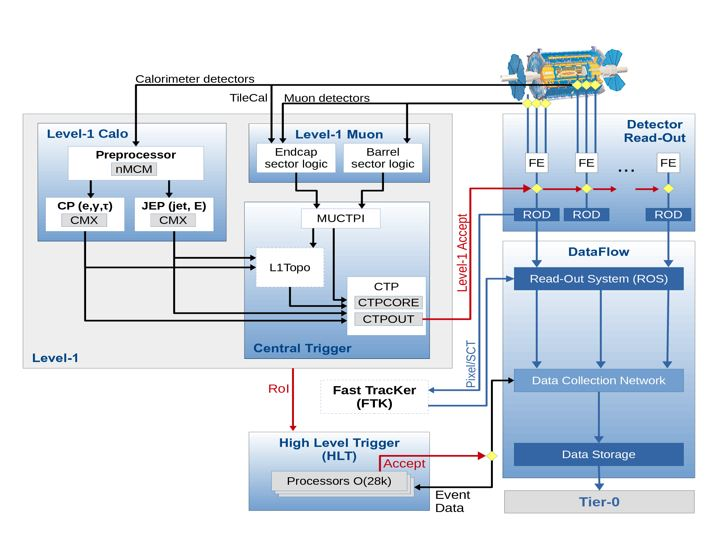
\includegraphics[width=0.95\textwidth]{figures/experiment/trigger.jpg}
    \caption{The ATLAS trigger logic in Run-2. Figure reproduced from Ref.~\cite{Ruiz-Martinez:2133909}.}
    \label{fig:trigger-scheme}
\end{figure}

The L1 trigger system reduces the data rate to approximately \SI{100}{\kilo\hertz}. It uses a subset of the full detector information to decide between keeping or discarding events within a latency of \SI{2.5}{\micro\second}. The L1 trigger decision is formed in the Central Trigger Processor (CTP), which receives information from the L1 calorimeter (L1 Calo) and the L1 muon (L1 Muon) triggers.

The L1 Calo trigger processes analogue signals from the electromagnetic and hadronic calorimeters, which are digitised and calibrated by a preprocessor system in approximately 7000 trigger towers with a granularity of \(\Delta \eta \times \Delta \phi = 0.1 \times 0.1\).
Electron, photon and hadronically decaying \(\tau\) lepton candidates with specified energy thresholds and isolation criteria\footnote{Isolation implies that the energetic particle must have a minimum angular separation from any other significant energy deposit in the same event.} are identified by the Cluster Processor (CP). A Jet/Energy-sum Processor (JEP) is able to reconstruct jet candidates and compute scalar and missing energy sums from trigger elements with \(\Delta \eta \times \Delta \phi = 0.2 \times 0.2\) granularity.
The L1 Muon trigger processes signals from three stations.

The L1 Muon trigger processes signals from either three stations of RPC chambers in the barrel region or from three stations of TGC chambers in the end-cap. The principle underpinning the muon trigger is a coincidence of hits in the different trigger stations within the road of a muon candidate. The hit in the trigger chamber layer, which is referred to as the pivot plane, defines the infinite momentum track as the connecting line to the interaction point. As the muon candidate's \(p_{\text{T}}\) affects the curvature and consequently the width of the muon road, the deviation of a hit in other chamber layers from the infinite momentum track is used for a quick momentum estimate through a programmable coincidence logic. Three low-\(p_{\text{T}}\) thresholds (\SI{4}{\giga\electronvolt}, \SI{6}{\giga\electronvolt}, and \SI{10}{\giga\electronvolt}) are defined by coincidence windows using information from two trigger chamber layers. In addition, three high-\(p_{\text{T}}\) thresholds (\SI{11}{\giga\electronvolt}, \SI{15}{\giga\electronvolt}, and \SI{20}{\giga\electronvolt}) are defined by taking into account additional coincidence requirements with regard to the third layer.
The trigger signals from the barrel and end-cap triggers are combined into a set of six threshold multiplicities for each bunch crossing in the muon to CTP interface and passed on to the CTP.

Events accepted by the L1 trigger are buffered in the Read-Out System (ROS), awaiting further confirmation from the HLT.
The HLT decision is evaluated by a computing farm, which can run reconstruction algorithms with the same precision used in the offline reconstruction, with access to the event information in full granularity. It receives Region-of-Interest (RoI) information, consisting of essential features identified by the L1 trigger and the geographical coordinates of those regions within the detector where its selection process has identified those features. These form a starting point for the HLT algorithms. Their significantly better particle identification and momentum resolution sharpens the HLT decision and thus reduces the final data-taking rate to approximately \SI{200}{\hertz}.

\subsection{Grid computing}
\label{sec:experiment:ATLAS:computing}
Large-scale computing infrastructure is required to analyse a large amount of data recorded by the LHC experiments.
The Worldwide LHC Computing Grid (WLCG) is designed to preserve, distribute and analyse LHC collision data. It is a distributed computing grid, consisting of more than \num{160} computing centres in more than 40 countries. Different tiers hierarchically structure the role of  computing centres:
\begin{itemize}
    \item The Tier-0 centre is located at the CERN data centre and is responsible for the first-pass reconstruction.
    \item The thirteen Tier-1 centres receive raw data and reconstruction output from Tier-0 and are responsible for the safe-keeping of a proportional share of data and simulations and large-scale reprocessing.
    \item The over 160 Tier-2 centres are typically hosted by universities and other scientific institutes. They provide storage and adequate computing power for specific analysis tasks.
    \item Tier-3 resources refer to computing clusters offered by research institutions to individual users. There is no formal engagement between WLCG and Tier 3 resources, but they often provide access to the respective WLCG sites.
\end{itemize}

